\documentclass[journal,12pt,twocolumn]{IEEEtran}
 \usepackage{setspace}
 \usepackage{gensymb}
 \usepackage{graphicx}
 \singlespacing
\graphicspath{ {/user/adarshsrivastava/desktop/Matrix Theory/Assignemnt_7} }
 \usepackage[cmex10]{amsmath}
 \usepackage{amsthm}
 \usepackage{hyperref}
 \usepackage{mathrsfs}
 \usepackage{txfonts}
 \usepackage{stfloats}
 \usepackage{bm}
 \usepackage{cite}
 \usepackage{cases}
 \usepackage{subfig}
 \usepackage{longtable}
 \usepackage{multirow}
 \usepackage{enumitem}
 \usepackage{mathtools}
 \usepackage{steinmetz}
 \usepackage{tikz}
 \usepackage{circuitikz}
 \usepackage{verbatim}
 \usepackage{tfrupee}
 \usepackage[breaklinks=true]{hyperref}
 \usepackage{tkz-euclide}
 \usetikzlibrary{calc,math}
 \usepackage{listings}
     \usepackage{color}                                            %%
     \usepackage{array}                                            %%
     \usepackage{longtable}                                        %%
     \usepackage{calc}                                             %%
     \usepackage{multirow}                                         %%
     \usepackage{hhline}                                           %%
     \usepackage{ifthen}                                           %%
     \usepackage{lscape}     
 \usepackage{multicol}
 \usepackage{chngcntr}
 \DeclareMathOperator*{\Res}{Res}
 \renewcommand\thesection{\arabic{section}}
 \renewcommand\thesubsection{\thesection.\arabic{subsection}}
 \renewcommand\thesubsubsection{\thesubsection.\arabic{subsubsection}}
 \renewcommand\thesectiondis{\arabic{section}}
 \renewcommand\thesubsectiondis{\thesectiondis.\arabic{subsection}}
 \renewcommand\thesubsubsectiondis{\thesubsectiondis.\arabic{subsubsection}}
 \hyphenation{op-tical net-works semi-conduc-tor}
 \def\inputGnumericTable{}                                 %%
 \lstset{
 %language=C,
 frame=single, 
 breaklines=true,
 columns=fullflexible
 }
 \begin{document}
 \newtheorem{theorem}{Theorem}[section]
 \newtheorem{problem}{Problem}
 \newtheorem{proposition}{Proposition}[section]
 \newtheorem{lemma}{Lemma}[section]
 \newtheorem{corollary}[theorem]{Corollary}
 \newtheorem{example}{Example}[section]
 \newtheorem{definition}[problem]{Definition}
 \newcommand{\BEQA}{\begin{eqnarray}}
 \newcommand{\EEQA}{\end{eqnarray}}
 \newcommand{\define}{\stackrel{\triangle}{=}}
 \bibliographystyle{IEEEtran}
 \providecommand{\mbf}{\mathbf}
 \providecommand{\pr}[1]{\ensuremath{\Pr\left(#1\right)}}
 \providecommand{\qfunc}[1]{\ensuremath{Q\left(#1\right)}}
 \providecommand{\sbrak}[1]{\ensuremath{{}\left[#1\right]}}
 \providecommand{\lsbrak}[1]{\ensuremath{{}\left[#1\right.}}
 \providecommand{\rsbrak}[1]{\ensuremath{{}\left.#1\right]}}
 \providecommand{\brak}[1]{\ensuremath{\left(#1\right)}}
 \providecommand{\lbrak}[1]{\ensuremath{\left(#1\right.}}
 \providecommand{\rbrak}[1]{\ensuremath{\left.#1\right)}}
 \providecommand{\cbrak}[1]{\ensuremath{\left\{#1\right\}}}
 \providecommand{\lcbrak}[1]{\ensuremath{\left\{#1\right.}}
 \providecommand{\rcbrak}[1]{\ensuremath{\left.#1\right\}}}
 \theoremstyle{remark}
 \newtheorem{rem}{Remark}
 \newcommand{\sgn}{\mathop{\mathrm{sgn}}}
 \providecommand{\abs}[1]{\left\vert#1\right\vert}
 \providecommand{\res}[1]{\Res\displaylimits_{#1}} 
 \providecommand{\norm}[1]{\left\lVert#1\right\rVert}
 %\providecommand{\norm}[1]{\lVert#1\rVert}
 \providecommand{\mtx}[1]{\mathbf{#1}}
 \providecommand{\mean}[1]{E\left[ #1 \right]}
 \providecommand{\fourier}{\overset{\mathcal{F}}{ \rightleftharpoons}}
 %\providecommand{\hilbert}{\overset{\mathcal{H}}{ \rightleftharpoons}}
 \providecommand{\system}{\overset{\mathcal{H}}{ \longleftrightarrow}}
 	%\newcommand{\solution}[2]{\textbf{Solution:}{#1}}
 \newcommand{\solution}{\noindent \textbf{Solution: }}
 \newcommand{\cosec}{\,\text{cosec}\,}
 \providecommand{\dec}[2]{\ensuremath{\overset{#1}{\underset{#2}{\gtrless}}}}
 \newcommand{\myvec}[1]{\ensuremath{\begin{pmatrix}#1\end{pmatrix}}}
 \newcommand{\mydet}[1]{\ensuremath{\begin{vmatrix}#1\end{vmatrix}}}
 \numberwithin{equation}{subsection}
 \makeatletter
 \@addtoreset{figure}{problem}
 \makeatother
 \let\StandardTheFigure\thefigure
 \let\vec\mathbf
 \renewcommand{\thefigure}{\theproblem}
 \def\putbox#1#2#3{\makebox[0in][l]{\makebox[#1][l]{}\raisebox{\baselineskip}[0in][0in]{\raisebox{#2}[0in][0in]{#3}}}}
      \def\rightbox#1{\makebox[0in][r]{#1}}
      \def\centbox#1{\makebox[0in]{#1}}
      \def\topbox#1{\raisebox{-\baselineskip}[0in][0in]{#1}}
      \def\midbox#1{\raisebox{-0.5\baselineskip}[0in][0in]{#1}}
 \vspace{3cm}
 \title{Assignment 7}
 \author{Adarsh Srivastava}
 \maketitle
 \newpage
 \bigskip
 %\renewcommand{\thefigure}{\theenumi}
 \renewcommand{\thetable}{\theenumi}
 The link to the solution is
 \begin{lstlisting}
  https://github.com/Adarsh1310/EE5609
 \end{lstlisting}
 \begin{abstract}
 This documents solves a problem based on curve and tangent.
 \end{abstract}
  \section{\textbf{Problem}}
Find the slope of the tangent to the curve y=$\frac{x-1}{x-2}$, x$\not=$2 at x=10.
  \section{\textbf{Solution}}
\begin{align}
y=\frac{x-1}{x-2}\label{2.1}
\end{align}
Equation \eqref{2.1} can be expressed as
\begin{align}
y(x-2)=x-1\\
yx-2y-x+1=0\label{2.0.3}
\end{align}
From above we can say,
\begin{align}
\vec{V}=\frac{1}{2}\myvec{0 & 1\\ 1 & 0}\\
\vec{u}=\myvec{-\frac{1}{2}&-1}\\
f=1
\end{align}
Now,
\begin{align}
\because \abs{V} = \mydet{0& \frac{1}{2} \\ \frac{1}{2} & 0} < 0,
\end{align}
\eqref{2.1} is the equation of a hyperbola. To verify that this we will find the the characteristic equation of $\vec{V}$.
\begin{align}
\mydet{\lambda \vec{I}-\vec{V}} = \mydet{\lambda  & \frac{1}{2}\\ \frac{1}{2} & \lambda } &= 0
\\
\implies \lambda^2 - 2\lambda + \frac{3}{4} &= 0
\label{2.0.13}
\end{align}
The eigenvalues are the roots of \eqref{2.0.13} given by
\begin{align}
\lambda_1 = \frac{1}{2}, \lambda_2 = -\frac{1}{2}
\label{2.0.14}
\end{align}
The eigenvector $\vec{p}$ is defined as
\begin{align}
\vec{V} \vec{p}&= \lambda \vec{p}
\\
\implies \brak{\lambda\vec{I}-\vec{V}}\vec{p} &=0
\end{align}
where $\lambda$ is the eigenvalue.  For $\lambda_1 = \frac{1}{2}$,
\begin{align}
\brak{\lambda_1\vec{I}-\vec{V}}
= \myvec{\frac{1}{2} & \frac{1}{2}
\\ \frac{1}{2} & \frac{1}{2}} 
\xleftrightarrow[R_1 \leftarrow 2R_1] {R_2\leftarrow R_2-R_1}\myvec{1 & 1 \\0 & 0 }  
\\
\implies \vec{p}_1 = \frac{1}{\sqrt{2}}\myvec{1 \\- 1}
\end{align}
Now,$\lambda$ is the eigenvalue.  For $\lambda_2 = -\frac{1}{2}$,
\begin{align}
\brak{\lambda_2\vec{I}-\vec{V}}
= \myvec{-\frac{1}{2} & \frac{1}{2}
\\ \frac{1}{2} & -\frac{1}{2}} 
\xleftrightarrow[R_1 \leftarrow 2R_1] {R_2\leftarrow R_2+R_1}\myvec{-1 & 1 \\0 & 0 }  
\\
\implies \vec{p}_2 = \frac{1}{\sqrt{2}}\myvec{1 \\ 1}
\end{align}
From Equations,
\begin{align}
\vec{V} &= \vec{P}\vec{D}\vec{P}^{-1}=\vec{P}\vec{D}\vec{P}^T \quad \because \vec{P}^{-1} = \vec{P}^{T}
\\
\text{or, } \vec{D} &= \vec{P}^T\vec{V}\vec{P}
\end{align}
We can say that
\begin{align}
\vec{P} & =\myvec{\vec{p}_1 & \vec{p}_2} = \frac{1}{\sqrt{2}}\myvec{1 & -1\\ 1 & 1}\\
 \vec{D} &= \myvec{\lambda_1 & 0 \\ 0 & \lambda_2} =\myvec{\frac{1}{2} & 0\\ 0 & -\frac{1}{2}}
\end{align}
\because \vec{u}^T\vec{V}^{-1}\vec{u}-f > 0 ,$there isn't a need to swap axes.$
$In hyperbola,
\begin{align}
\vec{c}=-\vec{V}^-1\vec{u}\\
axes=
\begin{cases}
\sqrt{\frac{\vec{u}^T\vec{V}^{-1}\vec{u}-f}{\lambda_1}}\\ \sqrt{\frac{f-\vec{u}^T\vec{V}^{-1}\vec{u}}{\lambda_2}}
\end{cases}
\end{align}$
$From above equations we can say that,
\begin{align}
\vec{c}=\myvec{-2\\-1}\\
\sqrt{\frac{\vec{u}^T\vec{V}^{-1}\vec{u}-f}{\lambda_1}}=\sqrt{2}\\
\sqrt{\frac{f-\vec{u}^T\vec{V}^{-1}\vec{u}}{\lambda_2}}=\sqrt{2}
\end{align}
with the standard hyperbola equation becoming
\begin{align}
\frac{x^2}{2}-\frac{y^2}{2} = 1,
\label{2.0.30}
\end{align}$
$Let us assume slope to be l,now finding the direction vector and normal vector of the tangent with slope l.
\begin{align}
\vec{m}=\myvec{1\\l}\label{2.0.27}\\
\vec{n}=\myvec{l\\-1}\label{2.0.28}
\end{align}$
$Now considering the equations to find point of contact
\begin{align} \vec{q} = \vec{V}^{-1}\brak{\kappa \vec{n}-\vec{u}}\label{2.0.33}
\\
\kappa = \pm \sqrt{\frac{\vec{u}^T\vec{V}^{-1}\vec{u}-f}{\vec{n}^T\vec{V}^{-1}\vec{n}}} \label{2.0.34}
\end{align}$
$By using \eqref{2.0.34}
\begin{align}
\kappa=\sqrt{-\frac{1}{4l}}
\end{align}
Now substituting this $\kappa$ in \eqref{2.0.33}
\begin{align}
\vec{q}=\myvec{-2\sqrt{-\frac{1}{4l}}+2\\2\sqrt{\frac{-l}{4}}+1}
\end{align}
We know that x=10.
\begin{align}
-2\sqrt{-\frac{1}{4l}}+2=10\\
-2\sqrt{-\frac{1}{4l}}=8\\
\sqrt{-\frac{1}{4l}}=4\\
-\frac{1}{4l}=16\\
l=-\frac{1}{64}
\end{align}$
$The slope of the tangent to the curve y=$\frac{x-1}{x-2}$, x$\not=$2 at x=10 is $\frac{1}{64}$.
So,from the above we can say that $\kappa$=4,-4 and from equation \eqref{2.0.27} and \eqref{2.0.28} direction and normal vectors will come out to be
\begin{align}
\vec{m}=\myvec{1\\-\frac{1}{64}}\\
\vec{n}=\myvec{-\frac{1}{64}\\-1}
\end{align}
Now using equation \eqref{2.0.33}
\begin{align}
\vec{q}_1 = \vec{V}^{-1}\brak{\kappa_1 \vec{n}-\vec{u}}\\
\vec{q}_1 = \myvec{0&2\\2&0}\brak{-4 \myvec{-\frac{1}{64}\\-1}-\myvec{-\frac{1}{2}\\-1}}\\
\vec{q}_1=\myvec{10\\ \frac{9}{8}}\\
\vec{q}_2 = \vec{V}^{-1}\brak{\kappa_2 \vec{n}-\vec{u}}\\
\vec{q}_2 = \myvec{0&2\\2&0}\brak{4 \myvec{-\frac{1}{64}\\-1}-\myvec{-\frac{1}{2}\\-1}}\\
\vec{q}_2=\myvec{-6\\ \frac{7}{8}}
\end{align}
  \begin{figure}[h!]
	\centering
	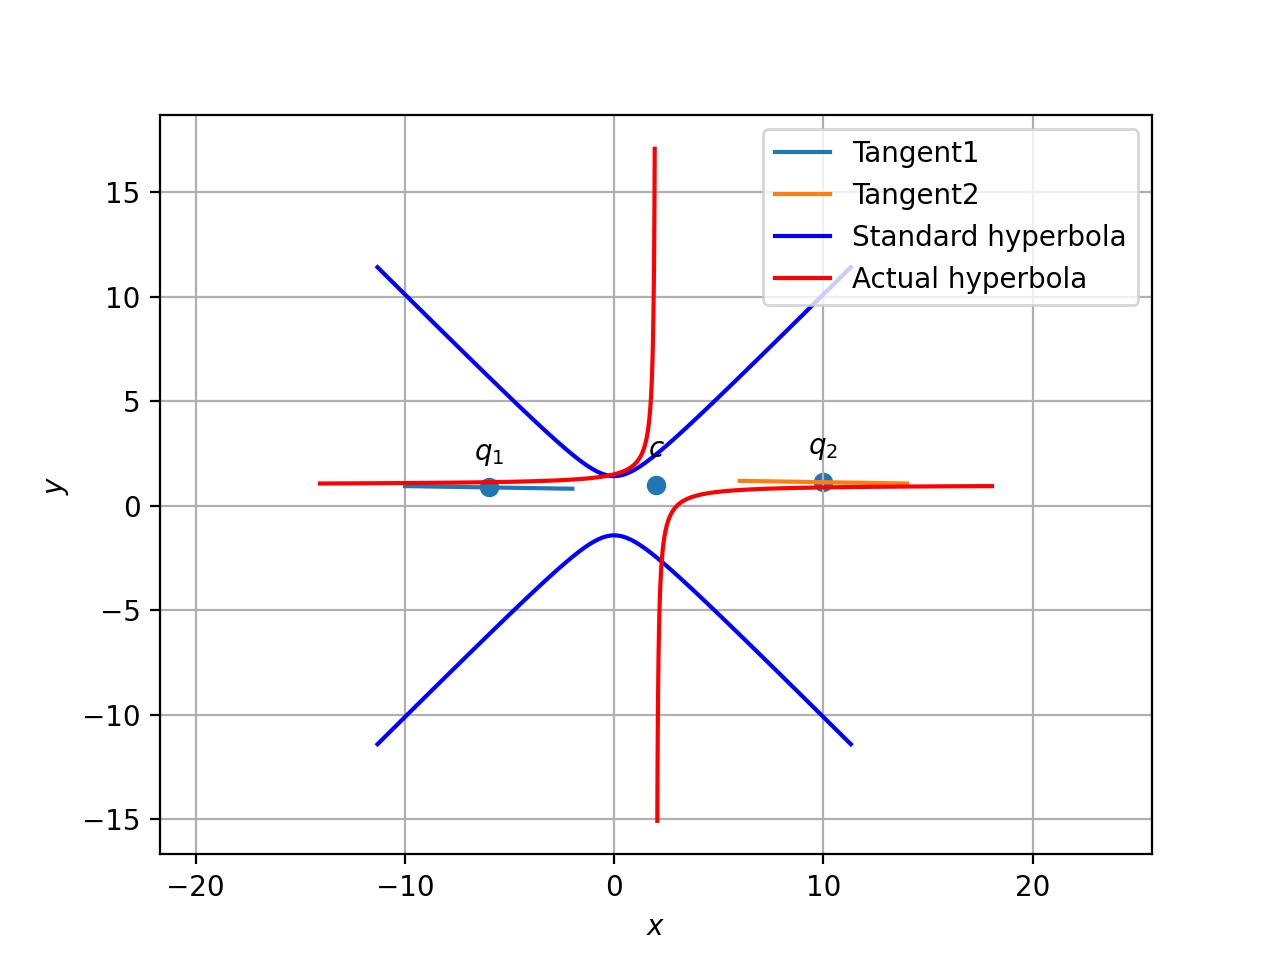
\includegraphics[width=\columnwidth]{Assignment_7.png}
	\caption{Tangent 2 shows the tangent}
	\label{myfig}
\end{figure}
 \end{document}
